\section{表面反射}\label{sec:表面反射}

当光入射到表面时,表面会散射该光,将其一部分反射回环境中。
有两个需要描述的效应以对反射建模:反射光的光谱分布和其方向分布。
例如,柠檬皮大都吸收了蓝波长的光而反射了大部分红和绿波长的光
(回想\reffig{5.1}中柠檬皮的反射SPD)。
因此,当用白光照射它时,其颜色是黄色。
无论从哪个方向观察,皮的颜色都相当一致,
但有的方向会有\keyindex{高光}{highlight}{}——会看见与其说黄色不如说白色的更亮区域
\sidenote{译者注:有高光区的柠檬照片。}。
\begin{marginfigure}
    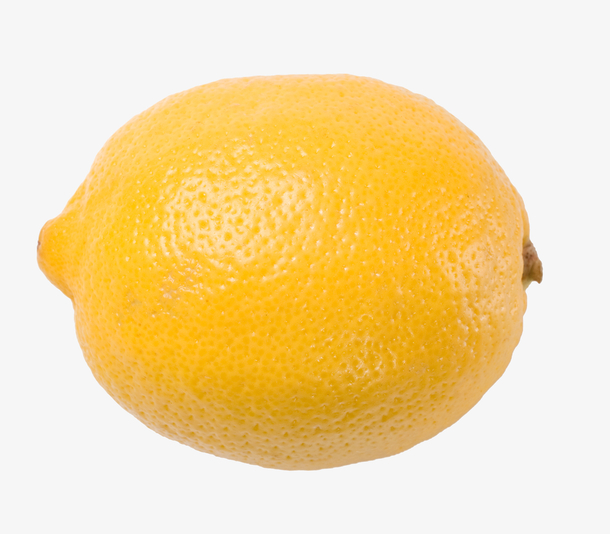
\includegraphics[width=\linewidth]{chap05/lemon.jpg}
\end{marginfigure}
相反,镜子一点反射的光几乎完全取决于观察方向。
在镜子的固定点上,当观察角度变化时,镜子反射的物体也随之变化。

来自\keyindex{半透明}{translucent}{}表面的反射更复杂;
从皮和叶子到蜡和液体的各种材料都
表现出\keyindex{次表面光传输}{subsurface light transport}{light transport光传输},
即进入表面一点的光在有一定距离的地方退出。
(例如考虑在一个人的嘴巴里开手电筒会让他的脸颊被照亮,
因为进入脸颊内侧的光穿过了皮肤并从脸上退出。)

有两种抽象来为光的反射描述这些机制:
\refsub{BRDF}和\refsub{BSSRDF}分别介绍的BRDF和BSSRDF。
BRDF描述一点的表面反射而忽略次表面光传输效应;
对于不受该传输机制明显影响的材料,
这一简化会减少报错并让渲染算法的实现高效得多。
BSSRDF推广了BRDF并描述来自半透明材料光反射的更一般设置。

\subsection{BRDF}\label{sub:BRDF}
\keyindex{双向反射分布函数}{bidirectional reflectance distribution function}{}(BRDF)
为描述来自表面的反射给出了形式。考虑\reffig{5.18}中的设置:
我们想知道,作为沿方向${\bm\omega}_{\mathrm{i}}$
入射辐亮度$L_{\mathrm{i}}({\bm p},{\bm\omega}_{\mathrm{i}})$的结果,
在朝向观察者的方向${\bm\omega}_{\mathrm{o}}$中
有多少辐射亮度$L_{\mathrm{o}}({\bm p},{\bm\omega}_{\mathrm{o}})$离开表面。
\begin{figure}[htbp]
    \centering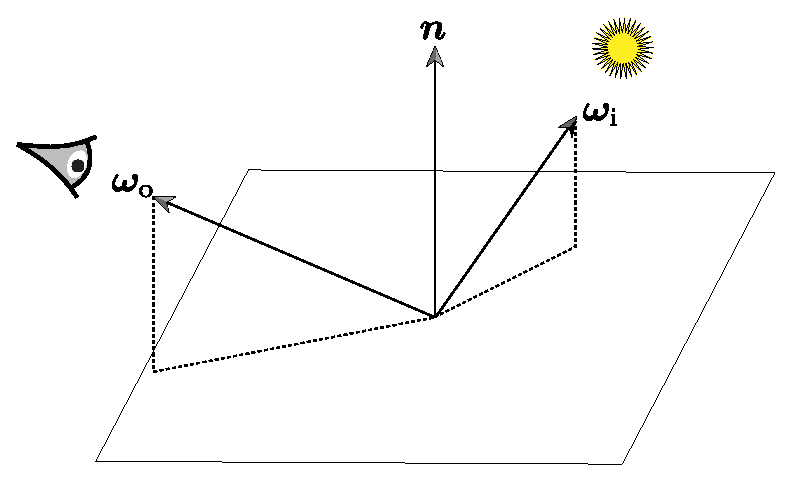
\includegraphics[width=0.5\linewidth]{chap05/BRDF.eps}
    \caption{BRDF。双向反射分布函数是在一对方向${\bm\omega}_{\mathrm{i}}$
        和${\bm\omega}_{\mathrm{o}}$上描述有多少沿${\bm\omega}_{\mathrm{i}}$
        入射的光从表面朝方向${\bm\omega}_{\mathrm{o}}$散射的4D函数。}
    \label{fig:5.18}
\end{figure}

如果方向${\bm\omega}_{\mathrm{i}}$视作方向的微分锥,则$\bm p$处的微分辐照度是
\begin{align}\label{eq:5.7}
    \mathrm{d}E({\bm p},{\bm\omega}_{\mathrm{i}})=L_{\mathrm{i}}({\bm p},{\bm\omega}_{\mathrm{i}})\cos\theta_{\mathrm{i}}\mathrm{d}{\bm\omega}_{\mathrm{i}}\, .
\end{align}

要被反射到方向${\bm\omega}_{\mathrm{o}}$的辐射亮度微分量取决于该辐射照度。
因为几何光学的线性假设,反射的微分辐射亮度正比于辐射照度
\begin{align*}
    \mathrm{d}L_{\mathrm{o}}({\bm p},{\bm\omega}_{\mathrm{o}})\propto\mathrm{d}E({\bm p},{\bm\omega}_{\mathrm{i}})\, .
\end{align*}

比例常数为这对特定方向${\bm\omega}_{\mathrm{i}}$和${\bm\omega}_{\mathrm{o}}$定义了曲面的BRDF:
\begin{align}\label{eq:5.8}
    f_{\mathrm{r}}({\bm p},{\bm \omega}_\mathrm{o},{\bm \omega}_\mathrm{i})=\frac{\mathrm{d}L_{\mathrm{o}}({\bm p},{\bm\omega}_{\mathrm{o}})}{\mathrm{d}E({\bm p},{\bm\omega}_{\mathrm{i}})}=\frac{\mathrm{d}L_{\mathrm{o}}({\bm p},{\bm\omega}_{\mathrm{o}})}{L_{\mathrm{i}}({\bm p},{\bm\omega}_{\mathrm{i}})\cos\theta_{\mathrm{i}}\mathrm{d}{\bm\omega}_{\mathrm{i}}}\, .
\end{align}

基于物理的BRDF有两个重要性质
\sidenote{译者注:事实上它还有非负性。}:
\begin{enumerate}
    \item \keyindex{互易性}{reciprocity}{}:对所有方向对${\bm\omega}_{\mathrm{i}}$和${\bm\omega}_{\mathrm{o}}$,
          $f_{\mathrm{r}}({\bm p},{\bm \omega}_\mathrm{i},{\bm \omega}_\mathrm{o})=f_{\mathrm{r}}({\bm p},{\bm \omega}_\mathrm{o},{\bm \omega}_\mathrm{i})$。
    \item {\sffamily 能量守恒}:光反射的总能量少于或等于入射光的能量。
          对于所有方向${\bm\omega}_{\mathrm{o}}$,
          \begin{align*}
              \int\limits_{H^2({\bm n})}f_{\mathrm{r}}({\bm p},{\bm \omega}_\mathrm{o},{\bm \omega}')\cos\theta'\mathrm{d}{\bm\omega}'\le1\, .
          \end{align*}
\end{enumerate}

曲面的\keyindex{双向透射分布函数}{bidirectional transmittance distribution function}{}
(BTDF)描述透射光的分布,可以用和BRDF一样的方法定义。
BTDF一般表示为$f_{\mathrm{t}}({\bm p},{\bm \omega}_\mathrm{o},{\bm \omega}_\mathrm{i})$,
其中${\bm\omega}_{\mathrm{i}}$和${\bm\omega}_{\mathrm{o}}$在绕$\bm p$的相对半球内。
要注意的是,BTDF不遵循上面定义的互异性;
我们将在\refsec{镜面反射与透射}和\refsub{非对称散射}详细讨论该问题。

为了等式的方便,我们把统一考虑时的BRDF和BTDF表示为$f({\bm p},{\bm \omega}_\mathrm{o},{\bm \omega}_\mathrm{i})$;
我们称之为\keyindex{双向散射分布函数}{bidirectional scattering distribution function}{}(BSFD)。
第\refchap{反射模型}将完全专注于描述对渲染有用的各种BSDF。

利用BSDF的定义,我们有
\begin{align*}
    \mathrm{d}L_{\mathrm{o}}({\bm p},{\bm\omega}_{\mathrm{o}})=f({\bm p},{\bm \omega}_\mathrm{o},{\bm \omega}_\mathrm{i})L_{\mathrm{i}}({\bm p},{\bm\omega}_{\mathrm{i}})|\cos\theta_{\mathrm{i}}|\mathrm{d}{\bm\omega}_{\mathrm{i}}\, .
\end{align*}
这里给项$\cos\theta_{\mathrm{i}}$加上了绝对值。
这样做是因为pbrt中曲面法线并没有调整为和${\bm\omega}_{\mathrm{i}}$位于曲面同侧
(许多其他渲染系统都这样做,但我们发现让它们留在原来\refvar{Shape}{}给出的自然朝向会更有用)。
这样做更容易一致地在系统别处运用如“假设曲面法线指向曲面外侧”那样的约定。
因此,像这样给项$\cos\theta_{\mathrm{i}}$加上绝对值保证了实际计算出所需的数量。
我们可以在绕$\bm p$的入射方向球内对该等式积分以计算由于各个方向对$\bm p$的照射
而得到的沿方向${\bm\omega}_{\mathrm{o}}$的出射辐亮度:
\begin{align}\label{eq:5.9}
    L_{\mathrm{o}}({\bm p},{\bm\omega}_{\mathrm{o}})=\int\limits_{S^2}f({\bm p},{\bm \omega}_\mathrm{o},{\bm \omega}_\mathrm{i})L_{\mathrm{i}}({\bm p},{\bm\omega}_{\mathrm{i}})|\cos\theta_{\mathrm{i}}|\mathrm{d}{\bm\omega}_{\mathrm{i}}\, .
\end{align}
这是渲染中的基本方程;它描述了一点的入射光分布
是怎样基于表面的散射性质转化为出射分布的。
当(像这里)球$S^2$作为积分域时它常常称为\keyindex{散射方程}{scattering equation}{},
当只在上半球$H^2({\bm n})$积分时则称\keyindex{反射方程}{reflection equation}{}。
\refchap{光传输I:表面反射}和\refchap{光传输III:双向方法}中积分例程的
关键任务之一就是计算场景中曲面上的点的该积分值。

\subsection{BSSRDF}\label{sub:BSSRDF}
\keyindex{双向散射表面反射分布函数}{bidirectional scattering surface reflectance distribution function}{}(BSSRDF)
是描述展现出明显程度次表面光传输的材料之散射的形式。
它是一个描述点${\bm p}_{\mathrm{o}}$在方向${\bm\omega}_{\mathrm{o}}$的出射微分辐亮度
与点${\bm p}_{\mathrm{i}}$来自方向${\bm\omega}_{\mathrm{i}}$的入射微分通量之比
的分布函数$S({\bm p}_{\mathrm{o}},{\bm\omega}_{\mathrm{o}},{\bm p}_{\mathrm{i}},{\bm\omega}_{\mathrm{i}})$
(\reffig{5.19}):
\begin{align}\label{eq:5.10}
    S({\bm p}_{\mathrm{o}},{\bm\omega}_{\mathrm{o}},{\bm p}_{\mathrm{i}},{\bm\omega}_{\mathrm{i}})=\frac{\mathrm{d}L_{\mathrm{o}}({\bm p}_{\mathrm{o}},{\bm\omega}_{\mathrm{o}})}{\mathrm{d}\varPhi({\bm p}_{\mathrm{i}},{\bm\omega}_{\mathrm{i}})}\, .
\end{align}
\begin{figure}[htbp]
    \centering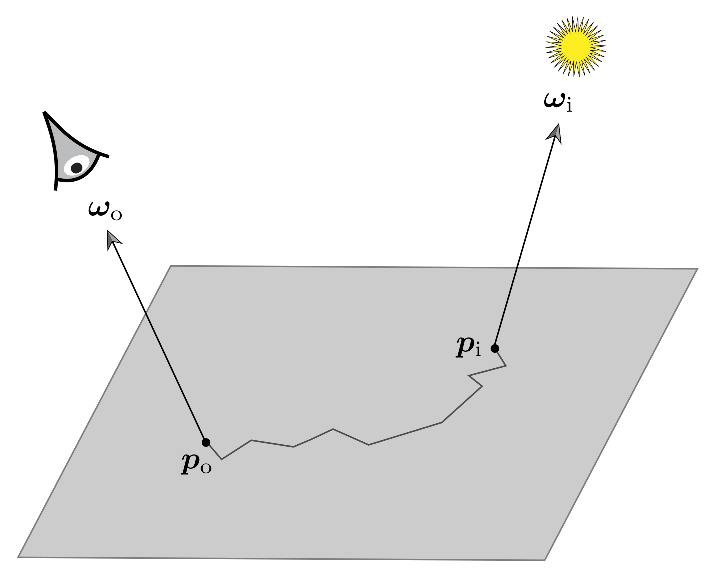
\includegraphics[width=0.5\linewidth]{chap05/BSSRDF.eps}
    \caption{双向散射表面反射分布函数推广了BSDF以考虑光在不同于其入射处的一点离开表面。
        尽管次表面光传输对许多真实世界物体的外观做出了巨大贡献,但它常常比BSDF更难算。}
    \label{fig:5.19}
\end{figure}

BSSRDF散射方程的推广需要在曲面面积\emph{以及}入射方向上积分,
将2D散射方程\refeq{5.9}转化为4D积分。
伴随着新增的两个积分维度,在渲染算法中使用它要复杂得多。
\begin{align}\label{eq:5.11}
    L_{\mathrm{o}}({\bm p}_{\mathrm{o}},{\bm\omega}_{\mathrm{o}})=\int\limits_A\int\limits_{H^2({\bm n})}S({\bm p}_{\mathrm{o}},{\bm\omega}_{\mathrm{o}},{\bm p}_{\mathrm{i}},{\bm\omega}_{\mathrm{i}})L_{\mathrm{i}}({\bm p}_{\mathrm{i}},{\bm\omega}_{\mathrm{i}})|\cos\theta_{\mathrm{i}}|\mathrm{d}{\bm\omega}_{\mathrm{i}}\mathrm{d}A\, .
\end{align}

随着点${\bm p}_{\mathrm{i}}$和${\bm p}_{\mathrm{o}}$的距离增加,$S$的值一般会减小。
这一事实对次表面散射算法的实现可以有很大帮助。

描述表面之下光传输的原则和介质中体积光传输方程一样,
由\refsec{转移方程}介绍的转移方程描述。
因此次表面散射基于和烟雾中光散射一样的效应,只是尺度更小。